\section{Flow Matching}

Like integer programming, flow matching is a problem that initially seems quite
niche, but actually has a lot of applications. In essence, given a weighted
graph, a `start' node and an `end' node, we want to compute the \textit{maximum
flow} through the graph from the source to the target. Imagine each edge is a
pipe between nodes, and liquid flows through the pipe. The weight of each edge
indicates how much liquid can flow through the graph, and a flow defines how
much liquid is flowing through each edge.

While flow matching, at first glance, seems only applicable to things like oil
pipelines and plumbing, we can actually map lots of problems onto graphs and
weighted edges.

\subsection{The stable marriage problem}

Given $n$ boys and $n$ girls, and a list for each boy and each girl of who they
would marry (this is binary; a yes/no thing), we want to come up with a $1-1$
pairing between the boys and the girls that produces the maximum number of
couples.

If we define that mathematically, then we let $G = (V, W, E)$, where $G$ is a
bipartite graph\marginpar{A bipartite graph is one who's nodes can be divided
into two disjoint sets, such that every edge in one of the sets connects to one
in the other.}, $V$ is the set of boys, $W$ is the set of girls and $E$ is the
set of edges. An edge from $v$ to $w$ indicates that $v$ and $w$ both would
marry each other.

$E' \subset E$ such that for all $v \in V$, there is at most one $w \in W$, and
for all $w \in W$, there is at most one $v \in V$. I.e, $E'$ is a matching
between the boys and girls, which is a subset of their preferences for each
other.

If every node has one edge (each item in $V$ and $W$ is incident to some $e \in
E'$), then the matching is perfect.

We can define the stable marriage problem to return \texttt{yes} if the input
graph has a perfect matching, and \texttt{no} otherwise.

A naive way of solving the problem is to iterate over each possible matching and
see if it is perfect:

\begin{lstlisting}[language=Java]
  boolean naiveSoln(Set<Node> boys, Set<Node> girls, Set<Edge> preferences) {
    if (boys.isEmpty()) {
      return girls.isEmpty();
    } else {
      Node randomBoy = boys.getRandomElement();
      for (Edge e : preferences) {
        if (e.from.equals(randomBoy)) {
          if (naiveSoln(
              boys.remove(e.from),
              girls.remove(e.to),
              preferences.remove(e))) {
            return true;
          }
        }
        return false;
      }
    }
  }
\end{lstlisting}

However, this is exponential in the size of $V$, since it might try every
combination of boy and girl, which is obviously exponential.

\subsection{Flow networks and flow matching}

A \textit{flow network} is a quintuple, as shown:

\begin{figure}[H]
  \centering
  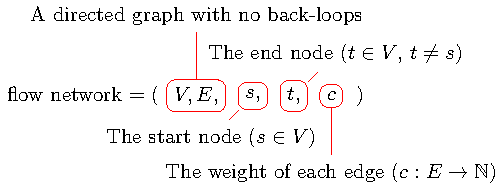
\includegraphics{equations/flow-network}
  \caption{Dissecting the definition of a flow network.}
  \label{fig:flow-network-definition}
\end{figure}

\textit{Back-loops} are a pair of edges that connect two nodes such that
$[(u,v),(v,u)]$

\begin{figure}[H]
  \centering
  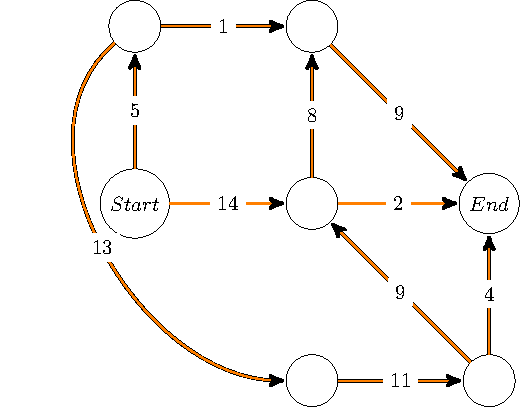
\includegraphics{diagrams/graph8}
  \caption{An example of a flow network. We assume that the start and edge 
    nodes have no incoming and outgoing edges respectively.}
  \label{fig:graph8}
\end{figure}

A \textbf{flow} over a flow network is a function $f : E \rightarrow
\mathbb{R^+}$ that has the following properties:

\begin{itemize}
  \item The net flow out of a node is zero.
  \item No edge exceeds its capacity ($f(u,v) \leq c(u,v)$).
  \item The \textit{value} of $f$ is the net flow out of the start node, or the
    net flow into the end node.
\end{itemize}

Our problem is that given a flow network $N$, we want to compute a flow for $N$
that has the maximum possible value (an optimal flow). If there is more than one
possible optimum flow, we don't mind which one is given.

In order to do this, we construct another graph (an \textit{auxiliary directed
graph}) from the one we're given. We construct the new graph by including all
the nodes, and following this rule for the edges; \textit{include an edge with
the value $c(u,v) - f(u,v)$ for all $u,v \in V$}.

This gives you the potential flow along each route. If an edge from $u$ to $v$
has a maximum capacity of $6$, but is carrying $2$, then in the auxiliary graph,
there should be an edge $(u,v)$ with a weight of $2$, and another from $(v,u)$
with a weight $4$ (since the flow can decrease by that much).

%TODO: Given example of creating an auxiliary graph

\subsubsection{The min-cut, max flow idea}

Remember, our end goal here is to get the maximum possible flow. The reason we
created an auxiliary graph in the first place, was because if there is a route
from the start node ($s$) to the end node ($t$) in it, then the flow is not
optimal.

Using this idea, we can make an algorithm to find the maximum flow:

\marginpar{I've made up some extra HashMap methods; increment and decrement. 
They assume that if the key isn't already associated with a value, the value 
was 0, and then they increment or decrement the value.}

\begin{lstlisting}[numbers=left,language=Java]
  Map<Edge, Integer> maximumFlow(List<Node> nodes, List<Edge> edges,
      Node start, Node end, Map<Edge, Integer> weight) {
    // Init the flow to all zeros
    Map<Edge, Integer> maxFlow = new HashMap<>();
    for (Edge e : edges) maxFlow.put(e, 0);
    // Iterate until we have a maximum flow
    while (true) {
      // Create the aux graph
      List<Edge> auxFlow = createAuxFlow(nodes, edges, flow, start, end);
      // Find the (possibly empty) path from the start to the end
      List<Edge> path = getPath(auxFlow, start, end);
      // If there is no path, then we're finished
      if (path.isEmpty()) break;
      else {
        for (Edge e : path) {
          // Increment each edge in the flow
          if (edges.contains(e)) maxFlow.increment(e);
          // If the edge isn't in the flow, decrement the edge going
          // the opposite way
          else maxFlow.decrement(e.reverse());
        }
      }
    }
    return maxFlow;
  }
\end{lstlisting}

If the flow network has integer capacities, then the optimal flow will have
integral values! This may be obvious in the above code, since the types are
integers, and we only ever increment or decrement.

We can find a path from any two nodes in linear time ($|V| + |E|$), as we do on
\texttt{Line 11}. If we define the constant $C$ to be the highest edge capacity,
then the maximum flow is $nC$, where $n$ is the number of nodes connected to the
start node, which could be $|V|$.

Therefore, the runtime of \texttt{maximumFlow} is $O(n(|V| + |E|)C) =
O(n(n+m)C)$

\subsubsection{Costs in flow networks}

What if we assigned every edge an associated cost that is charged per unit of
flow? We can add this to the definition of a flow network:

\begin{figure}[H]
  \centering
  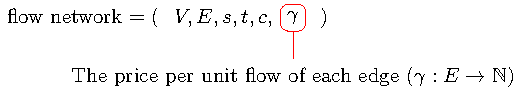
\includegraphics{equations/flow-network-costs}
  \label{fig:flow-network-definition-costs}
\end{figure}

%TODO: Add flow with costs

We can calculate the total cost of the flow to be:

\[
  \sum_{e \in E} f(e) \times \gamma(e)
\]

What if we want to find the maximum flow with the minimum cost? In fact, it is
possible to use the above \texttt{maximumFlow} algorithm to solve this, with
just a few small modifications; simply have the weight function $c$ take into
account $\gamma$:

\[
    c(e) = 
    \begin{cases}
        \gamma(e) & \text{if } (u,v) \text{is an edge in the aux graph, and in}
          ~E\\
        -\gamma(e) & \text{if } (u,v) \text{is an edge in the aux graph, and is
          not in}~E\\
    \end{cases}
\]

The only change we need to make on our flow finding algorithm is to find the
path from the start node to the end node using a minimal length:

\begin{lstlisting}[numbers=left,language=Java]
  Map<Edge, Integer> maximumFlow(List<Node> nodes, List<Edge> edges,
      Node start, Node end, Map<Edge, Integer> weight,
      Map<Edge, Integer> cost) {
    // Init the flow to all zeros
    Map<Edge, Integer> maxFlow = new HashMap<>();
    for (Edge e : edges) maxFlow.put(e, 0);
    // Iterate until we have a maximum flow
    while (true) {
      // Create the aux graph
      List<Edge> auxFlow = createAuxFlow(nodes, edges, flow, start, end);
      // Find the (possibly empty) path from the start to the end that has the
      // smallest cost
      List<Edge> path = getPath(auxFlow, start, end, cost);
      // If there is no path, then we're finished
      if (path.isEmpty()) break;
      else {
        for (Edge e : path) {
          // Increment each edge in the flow
          if (edges.contains(e)) maxFlow.increment(e);
          // If the edge isn't in the flow, decrement the edge going
          // the opposite way
          else maxFlow.decrement(e.reverse());
        }
      }
    }
    return maxFlow;
  }
\end{lstlisting}

This is the \textit{Busacker-Gowen algorithm}.

\subsection{Stable matching as a flow matching algorithm}

We can transform a matching problem into a flow matching problem as shown in
Figure~\ref{fig:matching-flow}.

\begin{figure}[H]
  \centering
  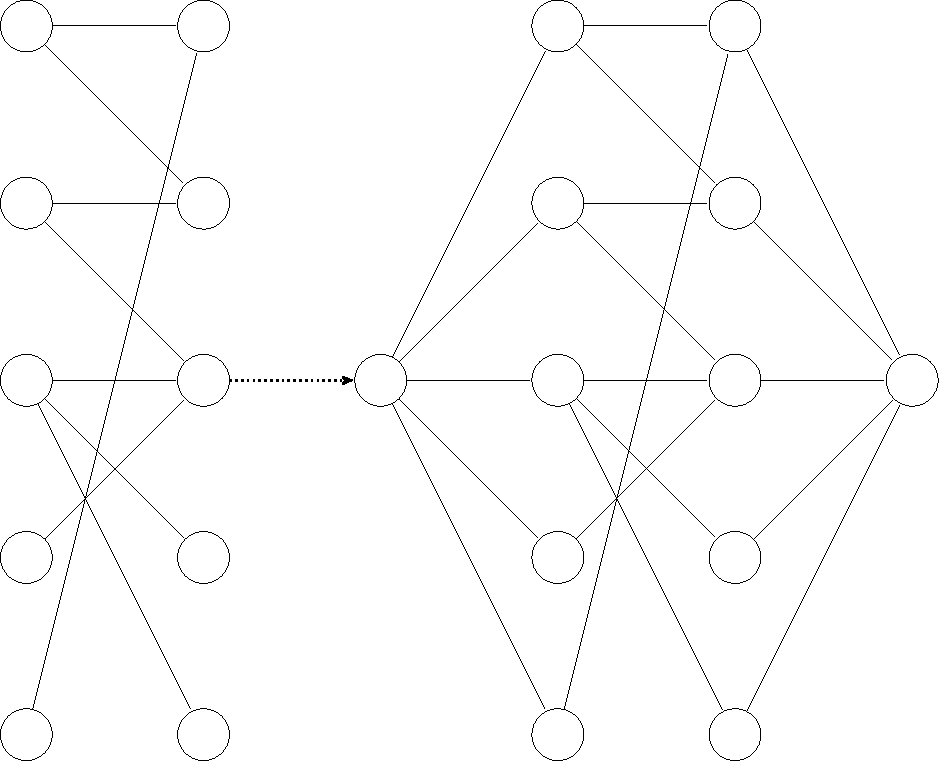
\includegraphics[width=0.6\textwidth]{diagrams/matching-flow}
  \caption{Here, a stable marriage problem (on the left, an edge indicates that
    both the boy and girl like each other) is mapped to a flow matching problem
    on the right.}
  \label{fig:matching-flow}
\end{figure}

We assume all the edge weights are $1$, and a perfect matching will be found iff
there is a flow from source to sink (the leftmost node to the rightmost node)
with a value $n$, where $n$ is the number of boys or girls. This runs on
$O(n(n+m))$ time!
